\documentclass{beamer}
\usepackage{graphicx, amsmath, amssymb, textcomp}

\newcommand{\pyplot}{\includegraphics[width=\textwidth, trim=60px 60px 60px 40px]}
\renewcommand{\vec}{\mathbf}

\newcommand{\bottomcite}{\let\thefootnote\relax\footnote}

\let\oldfootnotesize\footnotesize
\renewcommand*{\footnotesize}{\oldfootnotesize\tiny}


\begin{document}

\setbeamertemplate{navigation symbols}{}

\title{Effects of a superconducting lead endcap\\ on the magnetic field profile \\ for the nEDM search}
\author{Aritra Biswas\\Kellogg Radiation Laboratory\\Mentors: Brad Filippone, Simon Slutsky}
\maketitle

\begin{frame}
\frametitle{nEDM = neutron electric dipole moment}

    \begin{columns}

    \begin{column}{0.5\textwidth}
    \begin{itemize}
        \item distributed + and - charges inside neutron
        \item electric dipole moment (EDM) measures separation between
              centers of + and - charge
    \end{itemize}
    \end{column}
    
    \begin{column}{0.5\textwidth}
    \begin{figure}
    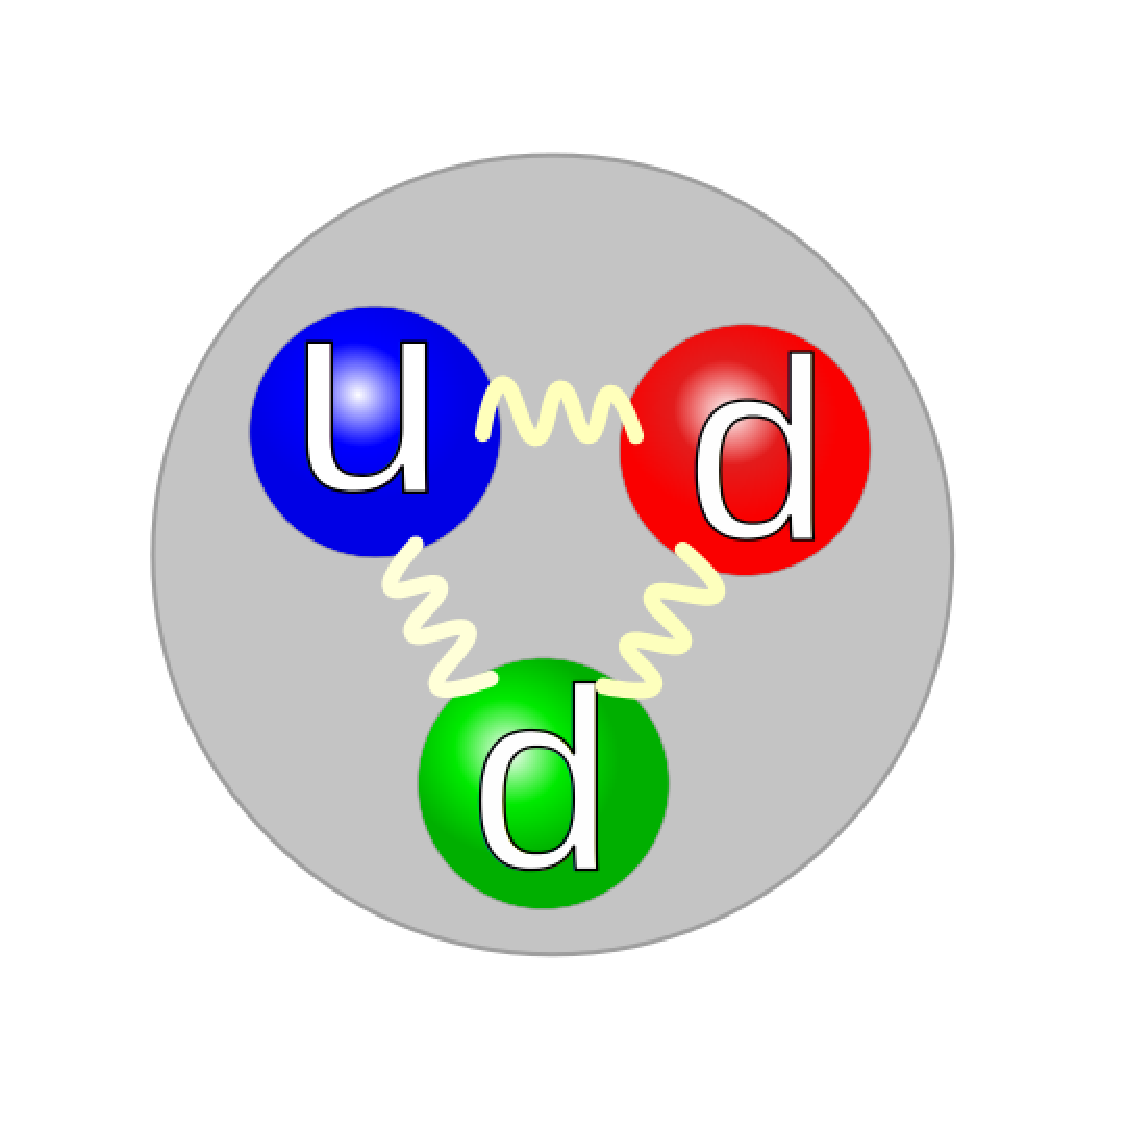
\includegraphics[width=\textwidth]{figures/neutron_quarks.eps}
    \end{figure}
    \end{column}

    \end{columns}

    \bottomcite{Horvath A. Quark structure neutron. Wikimedia.}

\end{frame}

\begin{frame}
\frametitle{why does the nEDM matter?}

    \begin{columns}
    
    \begin{column}{0.4\textwidth}
    \begin{figure}
    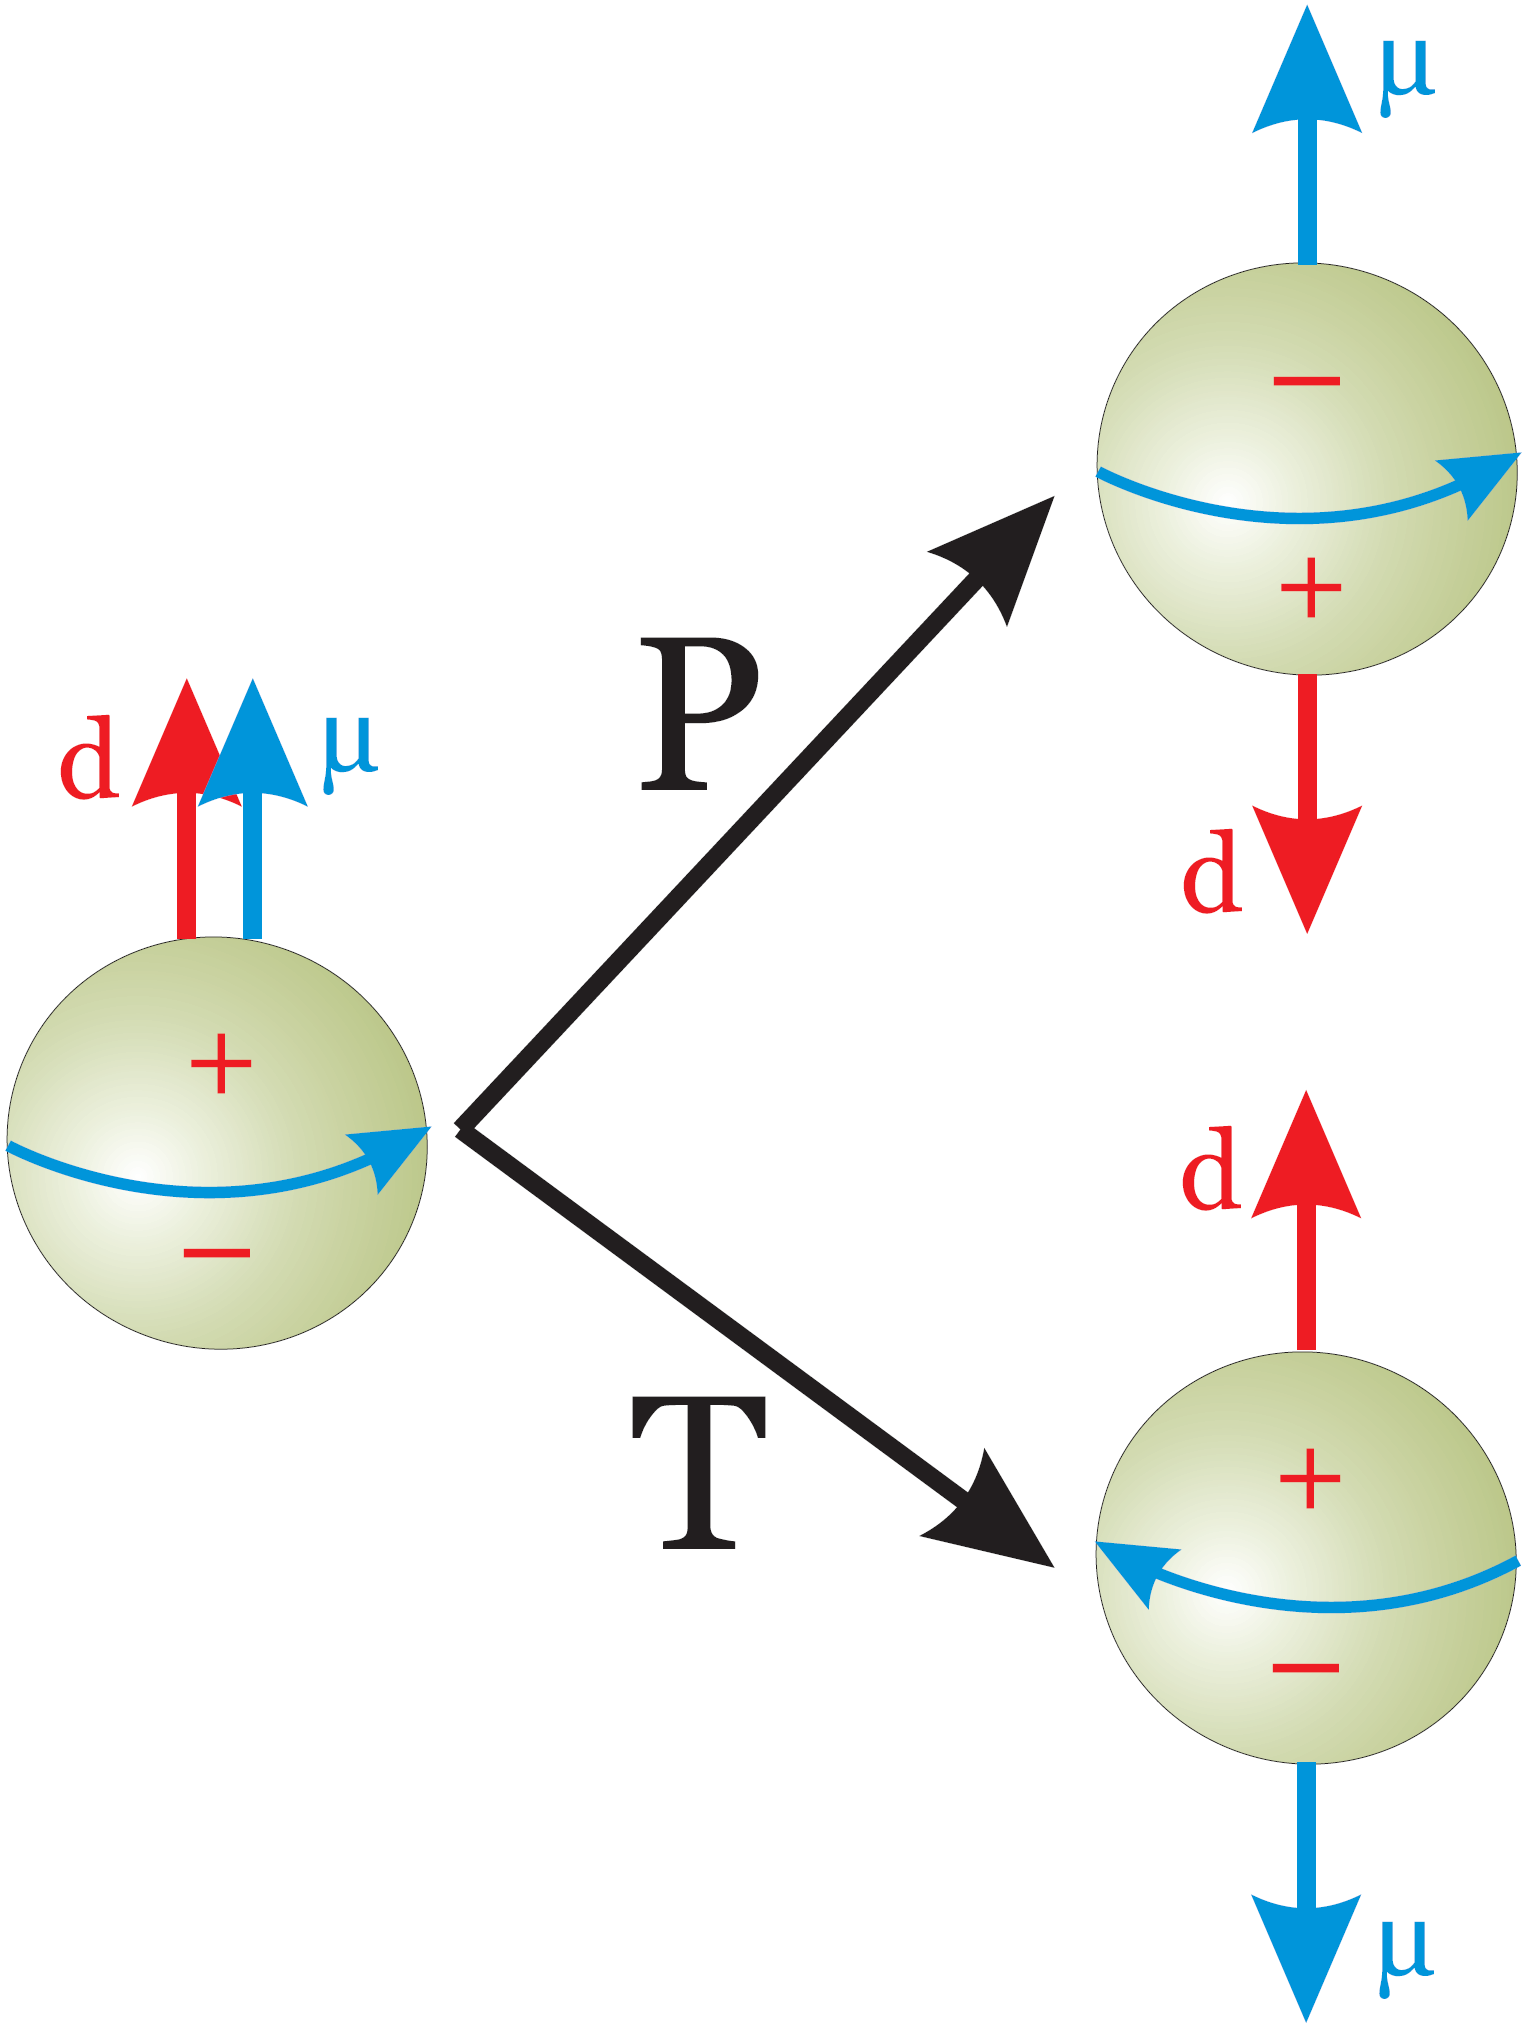
\includegraphics[width=\textwidth]{figures/nEDM_P_T_violation.png}
    \end{figure}
    \end{column}
   
    \begin{column}{0.6\textwidth}
    \begin{itemize} \pause
        \item $C: q \mapsto -q$ \pause
        \item $P: (t, x, y, z) \mapsto (t, -x, -y, -z)$ \pause
        \item $T: (t, x, y, z) \mapsto (-t, x, y, z)$ \pause
        \bigskip
        \item $CPT$ symmetry \\\pause + $P$ violation \\\pause + $T$ violation \\
        \pause $\Rightarrow$ $CP$ violation \pause
        \bigskip
        \item reformulations of Standard Model
        \item matter-antimatter asymmetry
    \end{itemize}
    \end{column}

    \end{columns}
    
    \bottomcite{Knecht A. 22 May 2008. Parity and time reversal violation. Wikimedia. Public domain.}

\end{frame}

\begin{frame}
\frametitle{how do we measure the nEDM?}

    \begin{itemize}
        \item put ultra-cold neutrons (UCN) in $\vec{E}$ and $\vec{B}$ fields \pause
        \item neutron's spin will precess at frequency $\omega$
        \begin{equation}
        \omega_{\uparrow\uparrow} = -\frac{\mu_n B + d_n E}{J\hbar}, \;\;\;
        \omega_{\uparrow\downarrow} = -\frac{\mu_n B - d_n E}{J\hbar}
        \end{equation} \pause
        \begin{equation}
        \Delta\omega = \pm\frac{2 \textcolor{blue}{d_n} E}{J\hbar} \pause \pm 
        \textcolor{red}{\Delta\omega_{geo}}
        \end{equation} \pause
        \item $\frac{\partial \vec{B}}{\partial (x,y,z)} \neq 0 \pause \Rightarrow
        \frac{\partial \vec{B}}{\partial t} \neq 0 \pause \Rightarrow$ $\vec{E}$ field
        \pause
        $\Rightarrow \textcolor{red}{\Delta\omega_{geo}}$ \pause
        \bigskip
        \item geometric phase $\Rightarrow$ false measurement! \pause
        \item engineering challenge: creating an uniform magnetic field
    \end{itemize}

    \bottomcite{Pendlebury et. al. Geometric-phase-induced false electric dipole moment signals
    for particles in traps. Phys. Rev. A. 70, 032102 (2004).}

\end{frame}

\begin{frame}
\frametitle{the half-scale model}

    \begin{columns}
    
    \begin{column}{0.5\textwidth}
    \begin{figure}
    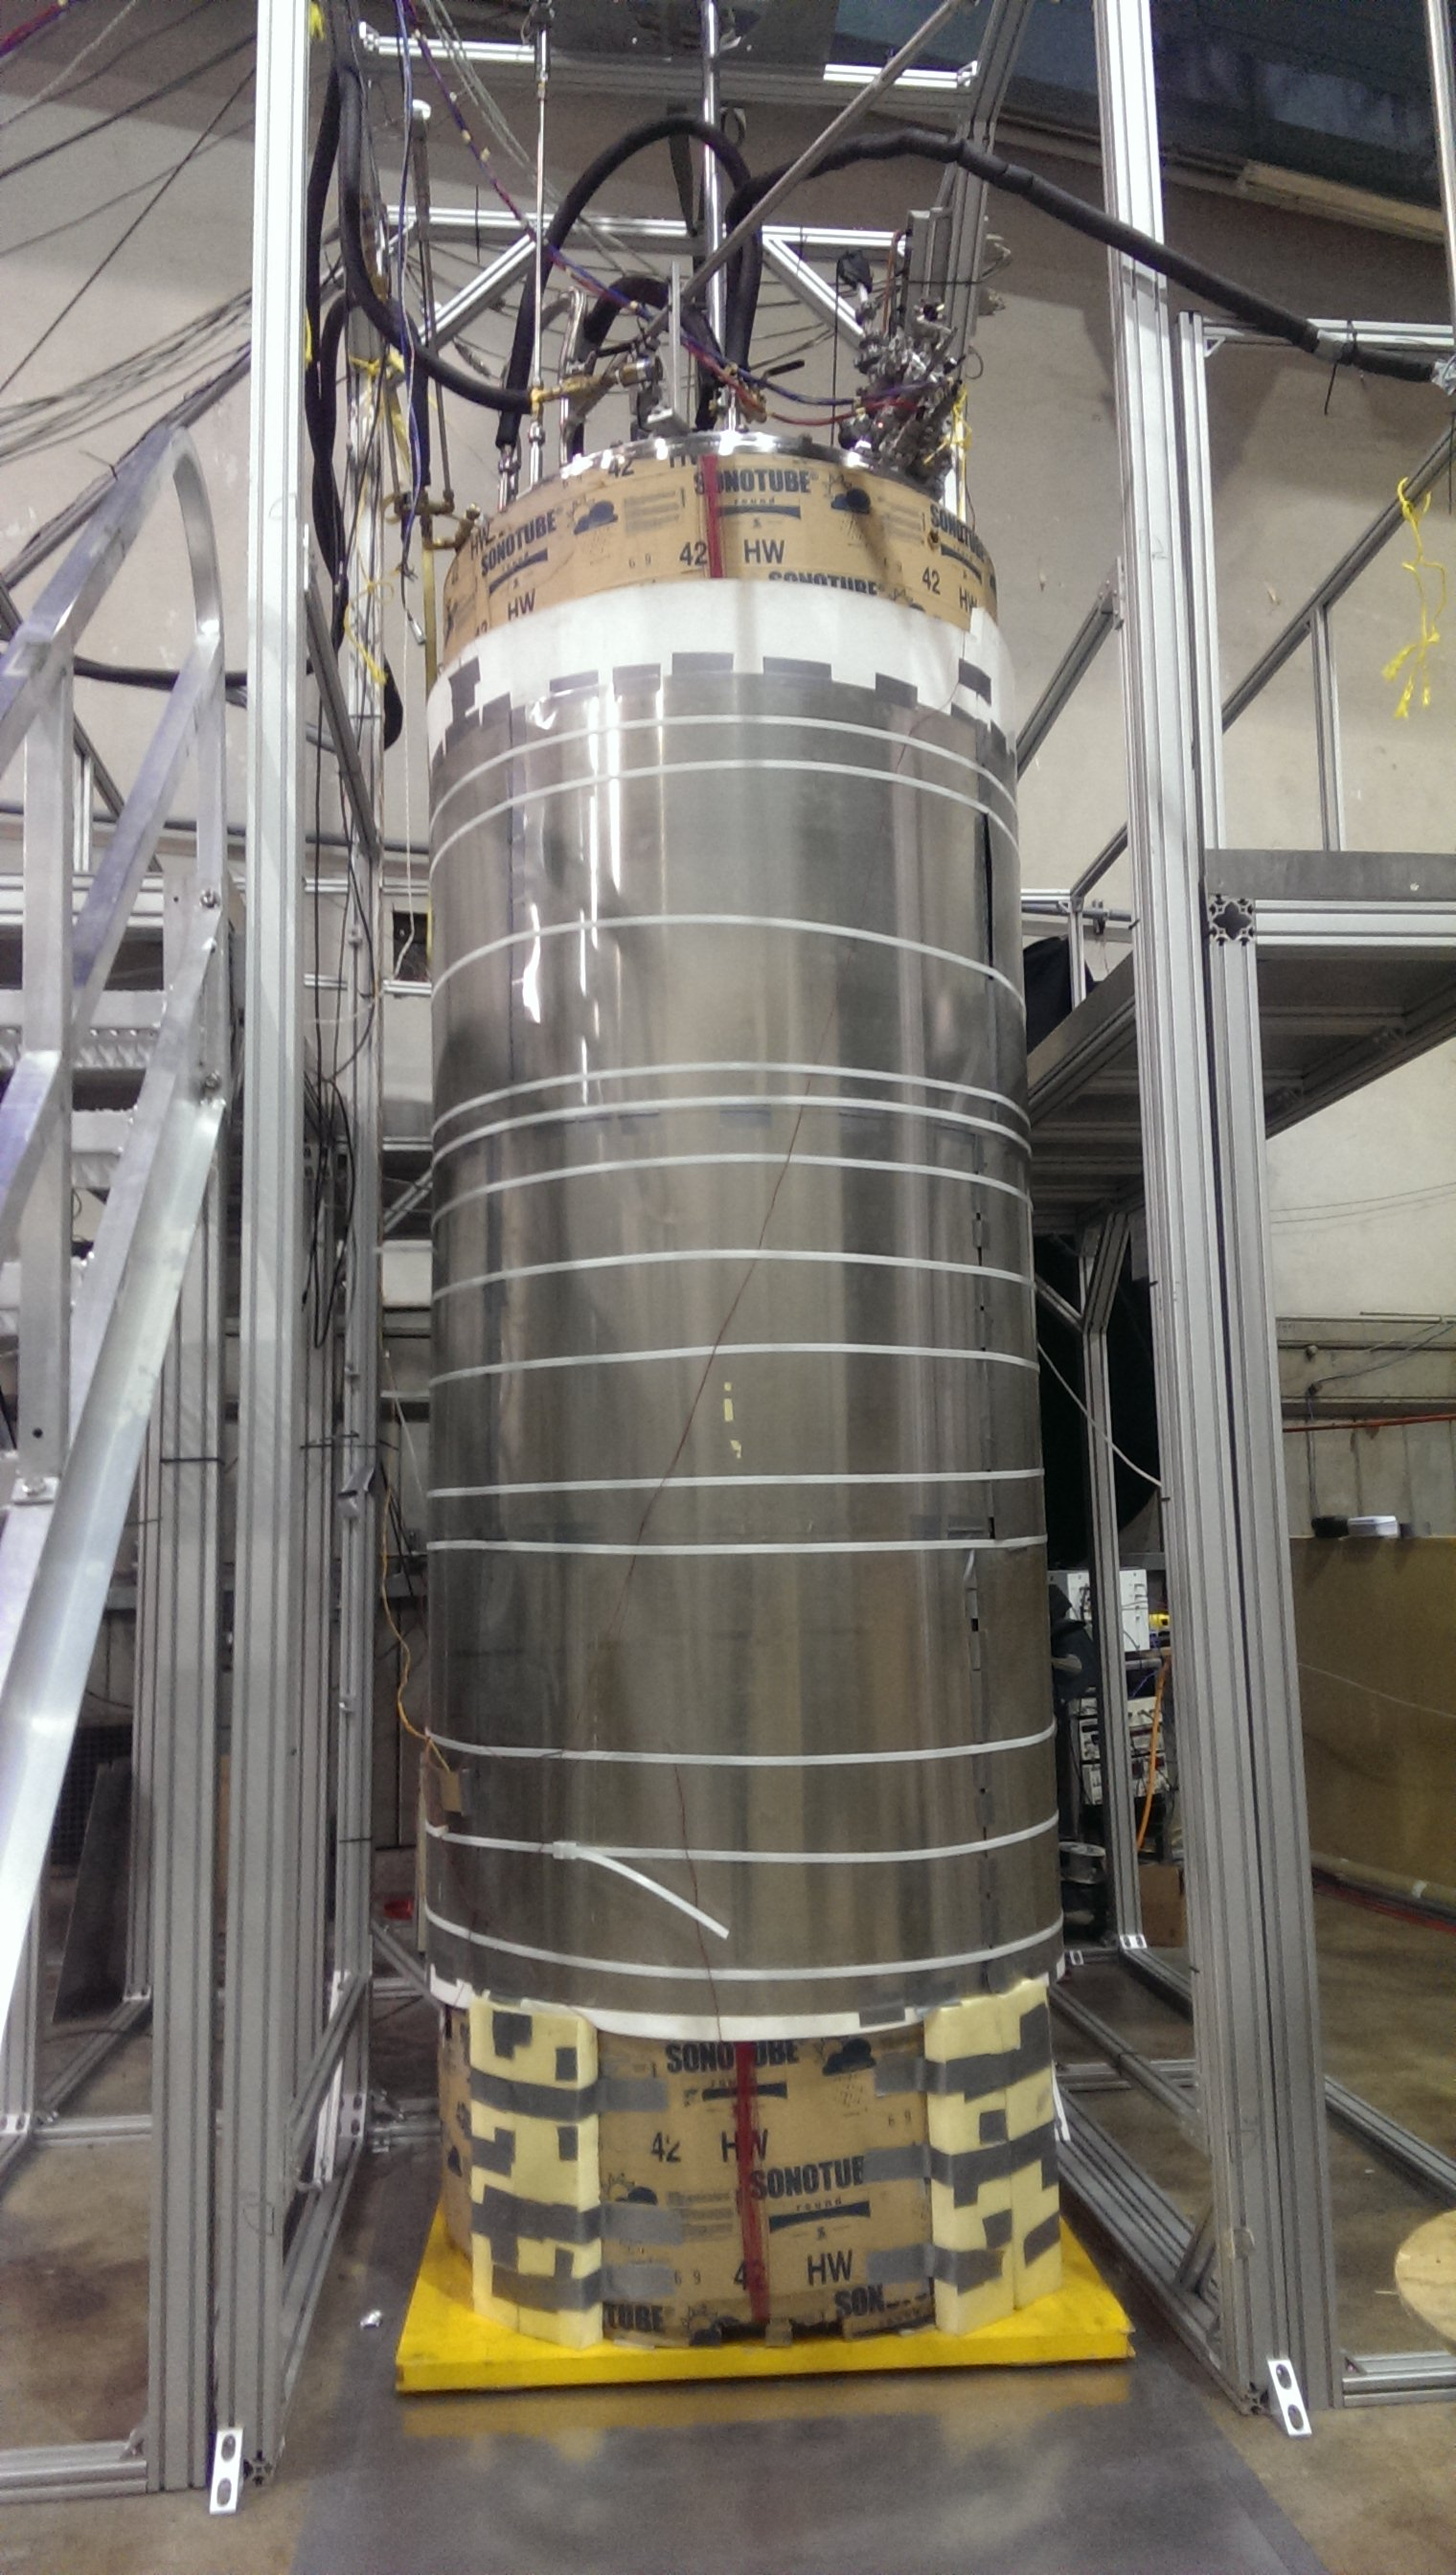
\includegraphics[width=0.9\textwidth]
    {figures/lab_picture.jpg}
    \end{figure}
    \end{column}
    
    \begin{column}{0.5\textwidth}
    \begin{itemize} \pause
        \item about 2 meters tall \pause
        \item inside a cryostat \\(cools to 4 K) \pause
        \item only creates $\vec{B}$ field;\\ no measurement cells \pause
        \item final experiment at Oak Ridge National Laboratory
    \end{itemize}
    \end{column}

    \end{columns}

\end{frame}

\begin{frame}
\frametitle{inside the half-scale model}

    \begin{columns}
    
    \begin{column}{0.5\textwidth}
    \begin{figure}
    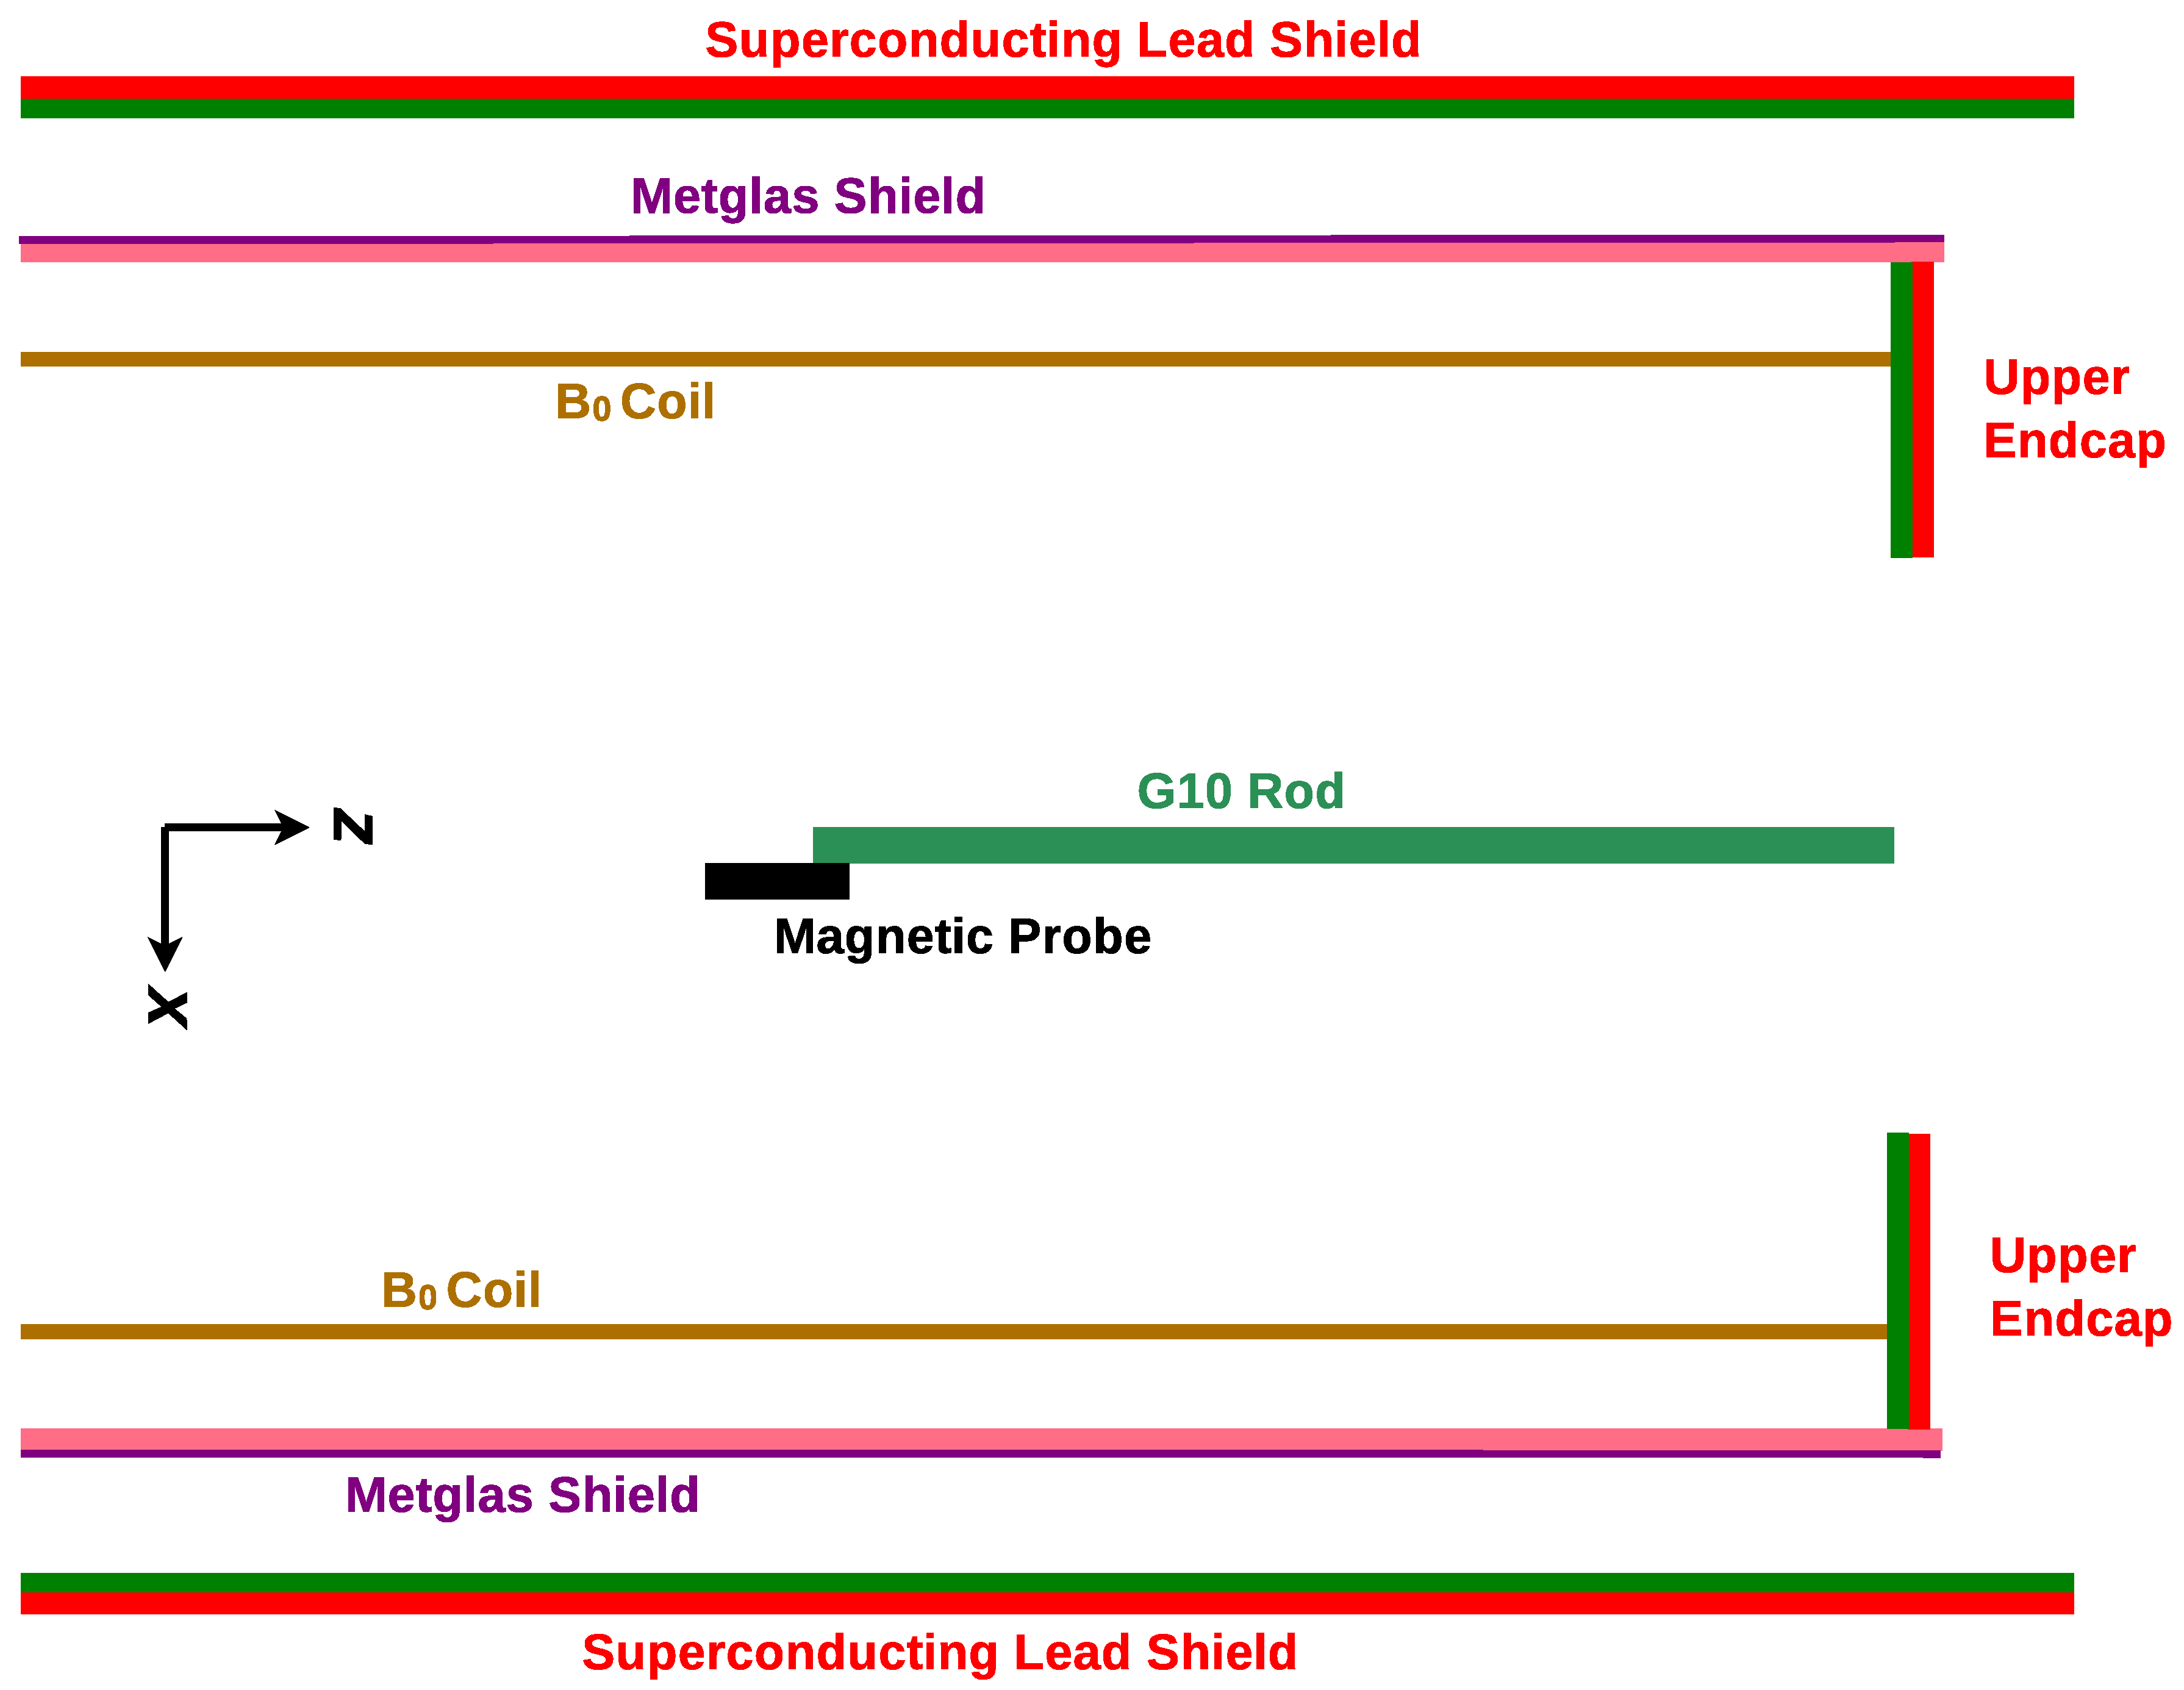
\includegraphics[width=\textwidth, angle=90, trim=70px 70px 70px 70px]
    {figures/simplified_structure.eps}
    \end{figure}
    \end{column}

    \pause

    \begin{column}{0.5\textwidth}
    \begin{itemize}
        \item $B_0$ coil: $\cos\theta$ coil geometry \pause
            \begin{itemize}
                \item $\vec{B}$ field in $x$ direction \pause
            \end{itemize}
        \bigskip
        \item ferromagnetic Metglas shield\pause
            \begin{itemize}
                \item high $\mu$ \pause
                %\item $\vec{B} \perp$ surface \pause
            \end{itemize}
        \item superconducting axial shield \pause
            \begin{itemize}
                \item $\mu = 0$ \pause
                %\item $\vec{B} \parallel$ surface \pause
            \end{itemize}
        \bigskip
        \item superconducting upper endcap
    \end{itemize}
    \end{column}

    \end{columns}

\end{frame}

\begin{frame}
\frametitle{edge effects and the superconducting endcap}

    \begin{columns}[b]
    
    \begin{column}{0.5\textwidth}
    \begin{figure}
    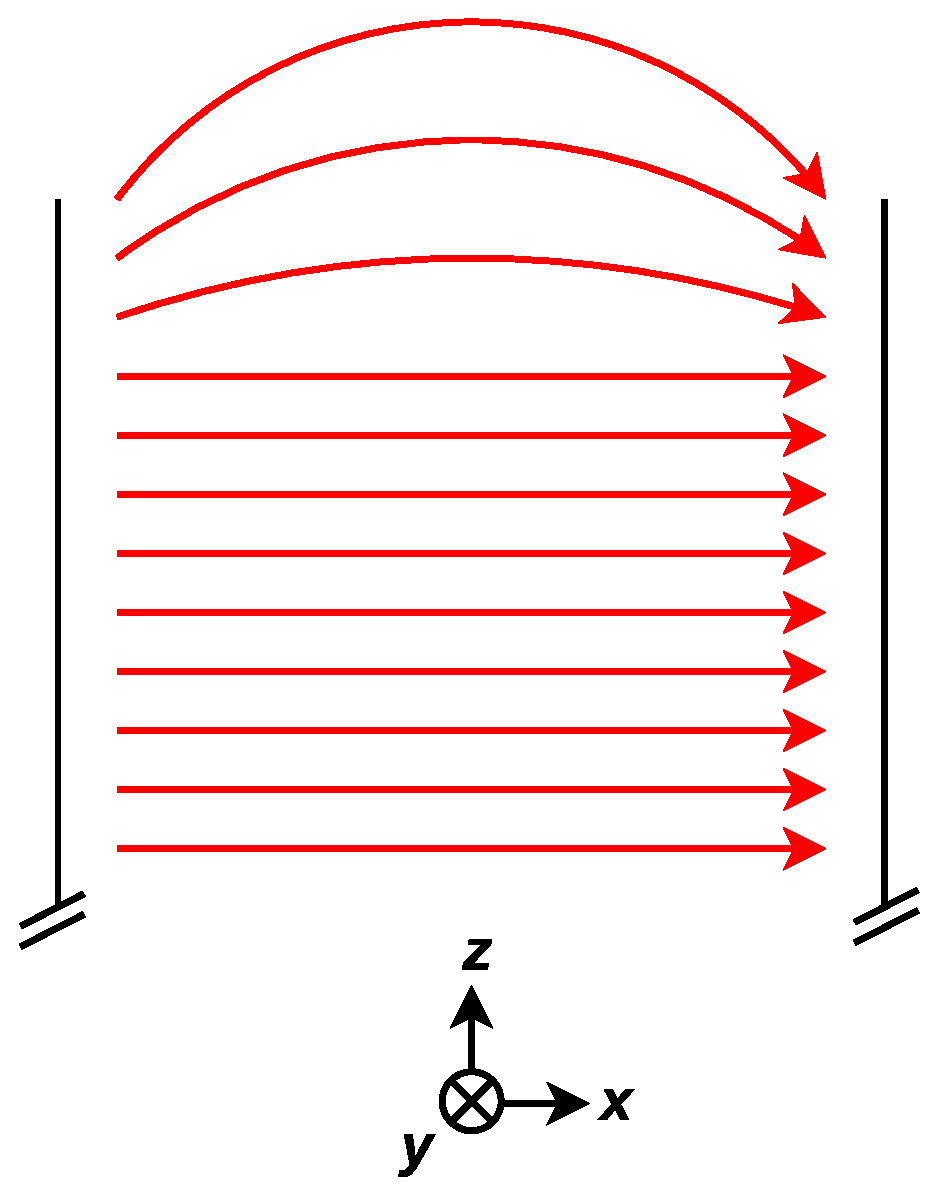
\includegraphics[width=\textwidth]
    {figures/field_noendcap.eps}
    \end{figure}
    \vspace{0pt}
    \end{column}

    \pause

    \begin{column}{0.5\textwidth}
    \begin{figure}
    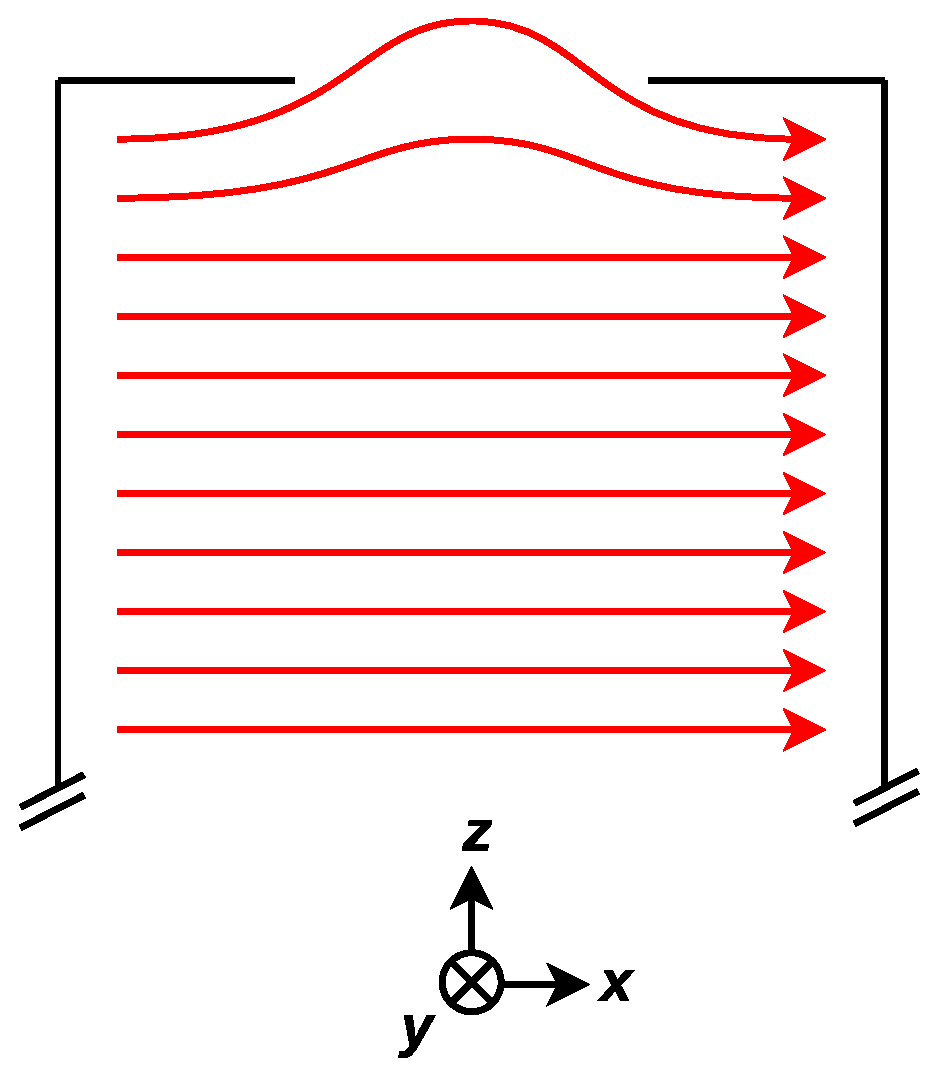
\includegraphics[width=\textwidth]
    {figures/field_endcap.eps}
    \end{figure}
    \vspace{0pt}
    \end{column}
    
\end{columns}

\end{frame}

%\begin{frame}
%\frametitle{analyzing the magnetic field profile}
%
%    \begin{itemize}
%        \item simulate experiment and calculate field
%        \item compare simulation and measurement in warm case
%        \item correct measurements
%        \item use simulation to predict effects of endcap
%        \item see whether measurements agree
%    \end{itemize}
%
%\end{frame}

%\begin{frame}
%\frametitle{configurations}
%
%    \begin{enumerate} \pause
%        \item axial shield normal, endcap normal \pause
%        \item axial shield SC, endcap normal \pause
%        \item axial shield SC, endcap SC \pause
%    \end{enumerate}
%
%    \bigskip
%
%    \begin{itemize}
%        \item simulate each configuration \pause
%        \item create each configuration using selective heating
%    \end{itemize}
%
%\end{frame}

\begin{frame}
\frametitle{simulations of endcap effect}

    \begin{center}
        \pyplot{figures/Bz_z_sim.eps}
    \end{center}

\end{frame}

\begin{frame}
\frametitle{correction: probe $x$ centering}

    \begin{center}
    \pyplot{../savedplots/manyx_Bz_z.eps}
    \end{center}

\end{frame}

\begin{frame}
\frametitle{correction: probe axis offset}

    \begin{columns}
    
    \begin{column}{0.5\textwidth}
    \begin{figure}
    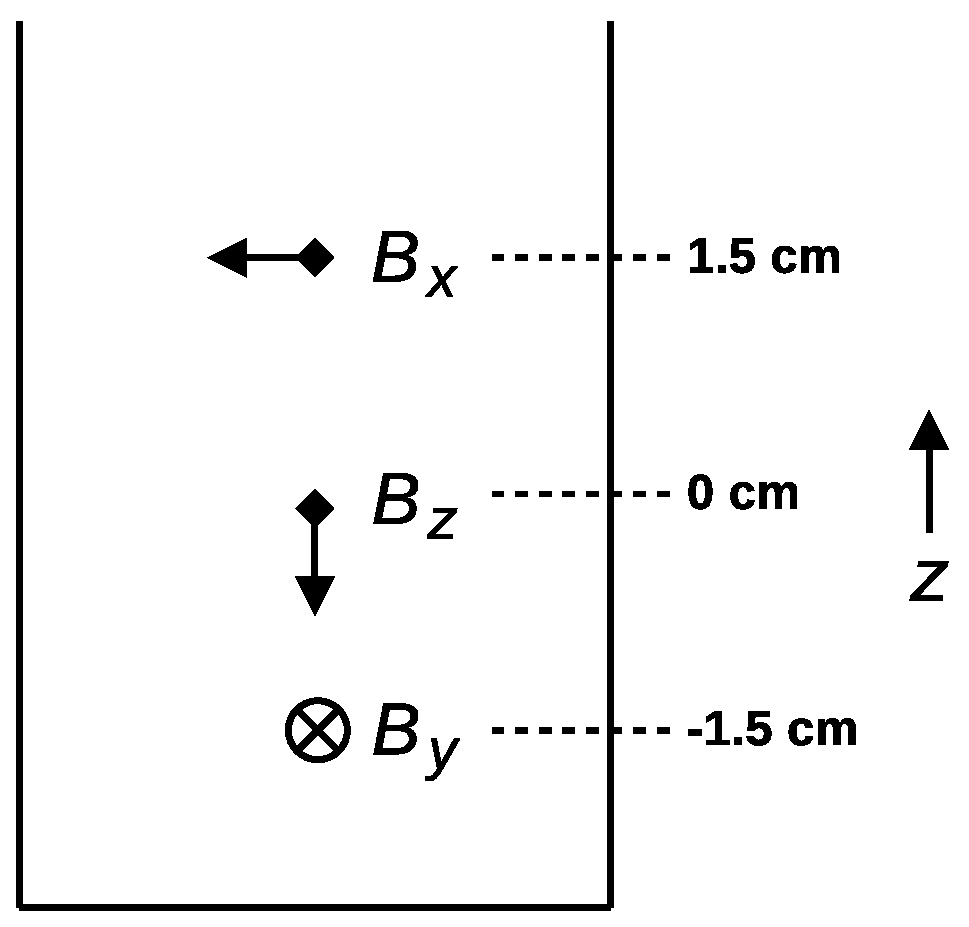
\includegraphics[width=\textwidth]
    {figures/probe.eps}
    \end{figure}
    \end{column}
    
    \begin{column}{0.5\textwidth}
    \begin{itemize}
        \item 3 separate 1-axis probes \pause
        \item incomplete vector map \pause
        \item need to store $z$-axis offset vector along with $z$ array \pause
    \end{itemize}
    \end{column}
   

    \end{columns}

\end{frame}

\begin{frame}
\frametitle{correction: probe tilt}
    
    \begin{center}
        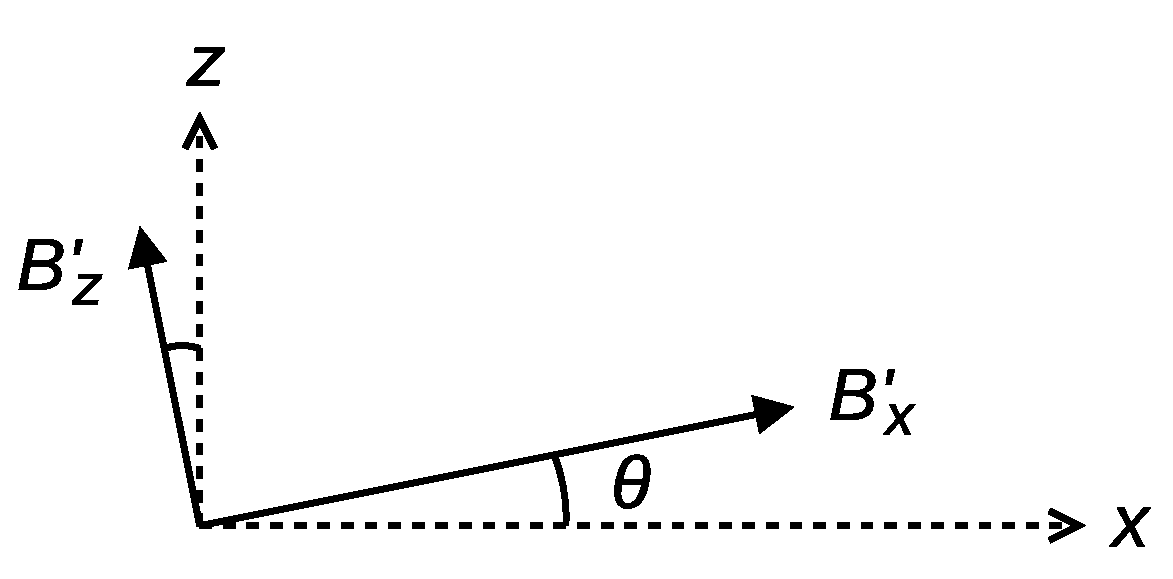
\includegraphics[width=0.5\textwidth]{figures/probe_tilt.eps}
    \end{center} \pause
    \begin{equation}
        B_x = B'_x \cos\theta - B'_z \sin\theta, \;\;\; B_z = B_z' \cos\theta + B_x' \sin\theta
    \end{equation}

    \pause

    \bigskip

    1. $\theta$ is small: \pause
    \begin{equation*}
        B_x = B'_x - B'_z \theta, \;\;\; B_z = B_z' + B_x' \theta
    \end{equation*} \pause
    2. $B_z = 0$ at center: \pause
    \begin{equation*}
        \theta = -\frac{B'_z}{B'_x}
    \end{equation*}

\end{frame}

\begin{frame}
\frametitle{comparison: axial shield normal, endcap normal}

    \begin{center}
        \pyplot{figures/normnorm_comp.eps}
    \end{center}
    
\end{frame}

\begin{frame}
\frametitle{comparison: axial shield SC, endcap normal}

    \begin{center}
        \pyplot{figures/SCnorm_comp_new.eps}
    \end{center}
    
\end{frame}

\begin{frame}
\frametitle{simulation: varying axial shield height}

    \begin{center}
        \pyplot{figures/axial_effect.eps}
    \end{center}

\end{frame}

\begin{frame}
\frametitle{simulation: varying axial shield height, with endcap}

    \begin{center}
        \pyplot{figures/axial_effect_endcap.eps}
    \end{center}

\end{frame}

\begin{frame}
\frametitle{comparison: axial shield SC, endcap SC}

    \begin{center}
        \pyplot{figures/SCSC_comp.eps}
    \end{center}
    
\end{frame}

\begin{frame}
\frametitle{analysis}

    \begin{itemize} \pause
        \item simulations are effective in predicting endcap behaviors \pause
        \item motivates further simulated studies with different endcap geometries \pause
        \item our endcap seems to shift the $B_z$ peak away from magnet center \pause
        \item axial shield effect is stronger when more of it is ``uncovered'' by the Metglas \pause
        \item SC endcap hides axial shield influence, even over small variation in height
    \end{itemize}

\end{frame}

\begin{frame}
\frametitle{ongoing and future work}

    \begin{itemize} \pause
        \item endcap will likely be effective in final experiment \pause
        \item new model with top and bottom endcaps \pause
        \item analysis of field gradients in measurement cell volumes
    \end{itemize}

\end{frame}

\begin{frame}
\frametitle{acknowledgments}

\begin{itemize}
    \item Mentor: Brad Filippone
    \item Co-mentor: Simon Slutsky
    \item Chris Swank, Chub Osthelder, Bob Carr
    \item Arthur R. Adams SFP Fellowship
    \item Caltech SURF Program
\end{itemize}

\end{frame}

\end{document}
